\chapter{DiscordBotを作ってみよう!}

\section{DiscordBotを作ってみよう}
\subsection{はじめに}
初めに今回何故DiscordのBotを作ろうと思ったかの経緯をお話しします。
私はDiscordで人とチャットをしている時に同じ会話が頻繁に続き、これBotで返事を返すようにしたら返事を返す手間が省けるし面白いのでは?と思ったのがBotを作ろうと思ったきっかけです。
発想がひどいって!?まあでも自分の発想したものを形にすることが面白いことだと思うので今回はそこには目を瞑りましょう…
もちろん自分が送ったメッセージに対してBotに返答させることもできるので、自分だけのオリジナルDiscordBotを作ってみましょう!

\subsection{何を作るのか}
Discordのサーバで特定のメッセージが来たら、特定のメッセージを返すDiscordのBotを作ります。

\section{実行環境・使用技術・ソースコードの管理}
\subsection*{実行環境}
調べる必要あり
\subsection*{使用技術等}
\begin{itemize}
  \item Python(discord.py)を使用
  \item Flaskを用いてWebサーバを構築
\end{itemize}
\subsection*{ソースコードの管理}
\begin{itemize}
  \item Git・GitHubを使用
  \item .envファイルをGitHubにアップロードしないようにする
\end{itemize}

\section{ローカル環境でBotが動作するようにする}
まずはローカル環境でBotが動作するようにしてみます。

\subsection{Botの作成・管理をする}
初めに機能などはまだついていないBotをDiscordのポータルサイトから作成します。
DiscordのBotの作り方(メモ)という記事の「1.Discord上のBotの作成」を見ながらBotを作成してみて下さい。
\footnote{引用した記事についての注釈を書く}。
同記事内の「2.Glitchでサーバーを作成」の部分は、今回Glitchは使用しないため行う必要はありません。

\subsection{Pythonの確認}
先ほど作成したBotをDiscordのサーバーに招待することができたらPythonが使えるかどうかの確認をしましょう。
Pythonを用いて先ほど作成したBotに機能をつけていきます。\\
今回はPythonの3.x系で実装します。\\
まずは、ローカル環境のPythonのバージョンを調べます。\\
\begin{shaded}
\begin{verbatim}
python --version
\end{verbatim}
\end{shaded}
この状態で2.x系のバージョンが出てくる場合は、下記のコマンドで3.x系のバージョンが出てくるか調べます。
\begin{shaded}
\begin{verbatim}
python3 --version
\end{verbatim}
\end{shaded}
今回はPython3.x系を利用するので3.xのバージョンが出たほうで実装を進めてください。\\
また、discord.pyについては3.8以降で動作します。3.8より前のバージョンが表示されている場合は、最新版のPythonをインストールしてください。

\section{本番環境へデプロイする}

\begin{tcolorbox}[breakable]
\begin{verbatim}
1  /* ここにはソースコードを書く */
2  #include<stdio.h>
3
4  int main(void)
5  {
6    printf("Hello, World!\n");
7    return 0;
8  }
9  /* breakableを付けるとこんな感じで改行にも対応できる */
\end{verbatim}
\end{tcolorbox}

\begin{shaded}
\begin{verbatim}
## ここにはコマンドを書く
$ echo "Hello, World!"
\end{verbatim}
\end{shaded}

図表はキャプションを付けたときに、先頭に「▲」や「▼」を付けるようにした。

\begin{table}[H]
  \centering
  \caption{表のサンプル}
  \begin{tabular}{|c|l|l|l|} \hline
    日本 & hoge & fuga & piyo \\ \hline
    アメリカ & foo & bar & baz \\ \hline
  \end{tabular}
  \label{table-sample0301}
\end{table}

\begin{figure}[H]
  \centering
  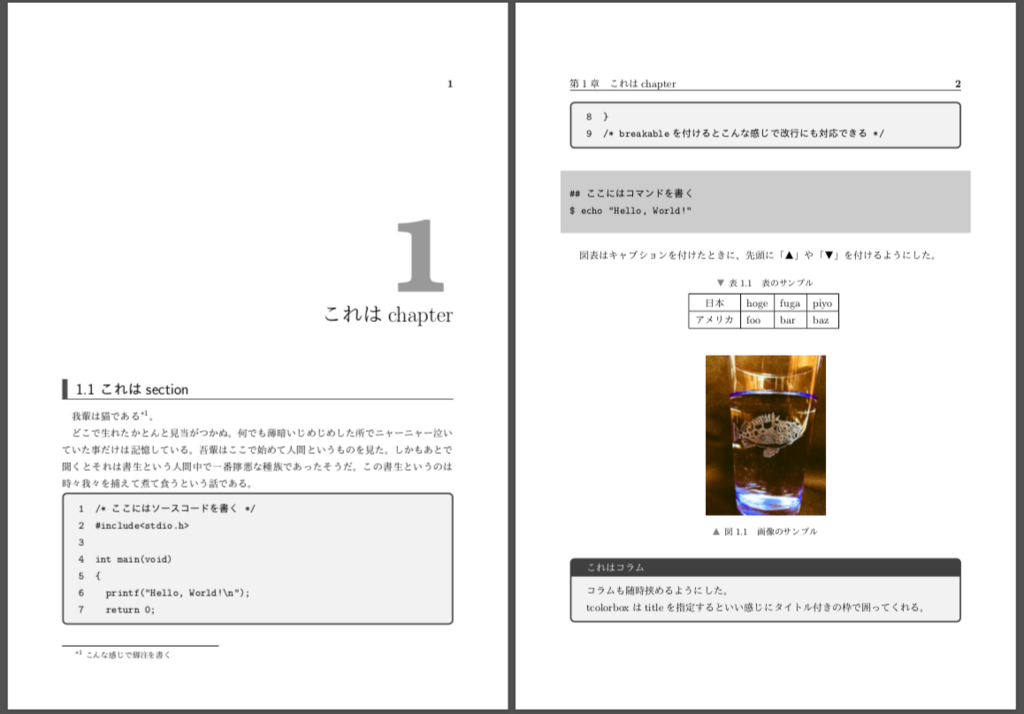
\includegraphics[width=4cm]{./image/03-Tech/chap1/sample.png}
  \caption{画像のサンプル}
  \label{figure-sample0301}
\end{figure}

\begin{tcolorbox}[title=これはコラム]
  コラムも随時挟めるようにした。

  tcolorboxはtitleを指定するといい感じにタイトル付きの枠で囲ってくれる。
\end{tcolorbox}